% !TEX root = /workplaces/database_talk/presentation/main.tex

\documentclass[aspectratio=169]{beamer}
\usepackage{import}

\import{preamble/}{packages.tex}
\import{preamble/}{base.tex}
\import{preamble/}{plot_settings.tex}

\title[ECC]{Занимательные практики использования базы данных PostgreSQL в RoR проектах}
\author[RNDSOFT]{ltv1304@yandex.ru}
\institute[]{RNDSOFT}
\date[]{\today}

\begin{document}
  
  \setbeamercolor{background canvas}{bg=RNDSorange} 
  \begin{frame}[plain]
    \centering
    \begin{minipage}{\dimexpr\textwidth\relax}
      \begin{tikzpicture}[remember picture, overlay]
        \node[anchor=north east, xshift=1em, yshift=-1em] at (current page.north east) {
          \includesvg[width=20em]{static/img/diamond.svg}
        };
      \end{tikzpicture}
      
      \centering
      \titlepage
    \end{minipage}
  \end{frame}

  \setbeamercolor{background canvas}{bg=white} 
  \part{Введение}
    \section{Литвинов Евгений}
      \begin{frame}
  % \vspace{2em}
  \begin{columns}
    \begin{column}{0.48\textwidth}
      % \begin{minipage}[\textheight]{\linewidth}
        % \vspace{1em}
        % {\fontsize{18}{21}\bfseries\selectfont Литвинов Евгений\par}
        % \vspace{4em}
        \begin{itemize}[label=\raisebox{0em}{
\includegraphics[width=1em]{static/img/arrow22.png}}]
            \item \vspace{0.5em} \textbf{2 года работаю в IT}
            \item \vspace{0.5em} \textbf{из них 2 года в RNDSoft}
            \item \vspace{0.5em} \textbf{из них 1 год и 9 месяцев в команде "Взыскатора"}
        \end{itemize}
      % \end{minipage}
    \end{column}
    \begin{column}{0.48\textwidth}
      % \begin{minipage}[\textheight]{\linewidth}
        % \vspace{3em}
        \begin{center}
          \begin{tikzpicture}
            \clip (0,0) circle (6em);
            \node[inner sep=0] at (0.2em,-2.5em) {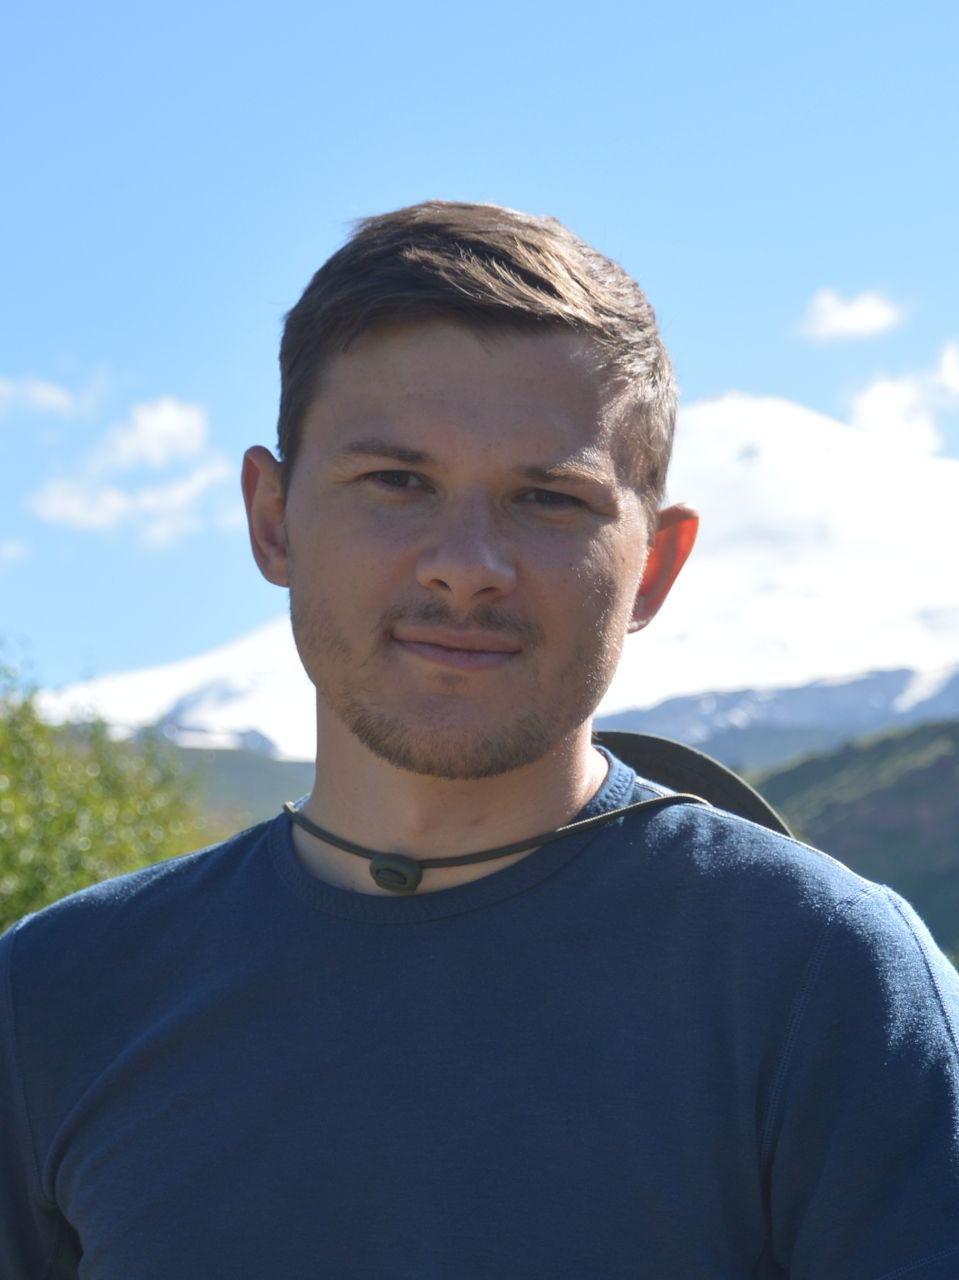
\includegraphics[width=0.8\textwidth]{static/img/speaker.jpg}};
          \end{tikzpicture}
        \end{center}
      % \end{minipage}
    \end{column}
\end{columns}
\end{frame}
    \section{План}
      \begin{frame}
  \begin{columns}
    \begin{column}{0.48\textwidth}
      \begin{minipage}[t][\textheight]{\linewidth}
        % \vspace{1em}
        % {\fontsize{18}{21}\bfseries План\par}
        \vfill
        \begin{tikzpicture}
          \fill[RNDScardBody, rounded corners=1em] (-2em,-2em) rectangle (12em,12em);
          \node at (5em,5em) {\includesvg[height=10em]{static/img/road_map.svg}};
        \end{tikzpicture}
        \vspace{1em}
        \end{minipage}
    \end{column}
    \begin{column}{0.48\textwidth}
      \begin{center}
        \begin{itemize}[label=\RNDSmarker]
          \item \vspace{0.5em} \textbf{Векторный поиск}\\
            про полнотекстовый поиск
          \item \vspace{0.5em} \textbf{Ряды} \\
            как сохранить историю изменений чего угодно
          \item \vspace{0.5em} \textbf{ExternalHash} \\
            выбрасывем хлам из базы данных 
        \end{itemize}
      \end{center}
    \end{column}
  \end{columns}

  \begin{tikzpicture}[remember picture, overlay]
    \node[fill=black, minimum height=1em, minimum width=0.5\paperwidth, anchor=south west, font=\ttfamily\color{green!70!black}\bfseries\large] 
      at ([yshift=0em]current page.south west) {\hspace{-4em} \# follow the white rabbit...};

  \end{tikzpicture}
\end{frame}


  \part{Основная часть}
    \section{Векторный поиск}
      \subsection{введение}
        \begin{frame}
  \bfseries Опасности, которые нас подстерегают при хранении больших JSON в БД?
  \normalfont
  \vspace{1em}
  \begin{itemize}[leftmargin=1em,itemsep=0.7em, label=\RNDSmarker]
    \item рост объёма хранилища
    \item дорогие бэкапы и восстановление
    \item сложность анализа
    \item память и скорость в Rails
    \item редкое использование тяжёлых данных
  \end{itemize}
\end{frame}
      \subsection{подходы}
        \begin{frame}
  % \vspace*{-0.5ex}
  % {\fontsize{18}{21}\bfseries Векторный поиск: подходы\par}
  % \vspace{1em} 
  \begin{columns} 
    \begin{column}{0.32\textwidth} 
      \begin{minipage}[\textheight]{\linewidth}
        \vspace{0.15\textheight} 
        \begin{tikzpicture} 
          \node[
            fill=RNDScardBody, 
            rounded corners=1em, 
            minimum width=\linewidth, minimum height=\linewidth, 
            align=center, 
            font=\ttfamily\color{RNDSorange}\LARGE\bfseries] (mainnode)
            {ILIKE}; 
        \end{tikzpicture} 
      \end{minipage} 
    \end{column} 
    \begin{column}{0.32\textwidth} 
      \begin{minipage}[\textheight]{\linewidth} 
        \vspace{0.15\textheight} 
        \begin{tikzpicture} 
          \node[
            fill=RNDScardBody, 
            rounded corners=1em, 
            minimum width=\linewidth, minimum height=\linewidth, 
            align=center, 
            font=\ttfamily\color{RNDSorange}\LARGE\bfseries] (mainnode)
            {tsvector};
          \node[
            star, star points=5, star point ratio=2.5, 
            fill=RNDSorange, minimum size=1em, scale=0.8, 
            anchor=north east, xshift=-1.5em, yshift=-1.5em
          ] at (mainnode.north east) {};
        \end{tikzpicture} 
      \end{minipage} 
    \end{column} 
    \begin{column}{0.32\textwidth} 
      \begin{minipage}[\textheight]{\linewidth} 
        \vspace{0.15\textheight} 
        \begin{tikzpicture} 
          \node[
            fill=RNDScardBody, 
            rounded corners=1em, 
            minimum width=\linewidth, minimum height=\linewidth, 
            align=center, 
            font=\ttfamily\color{RNDSorange}\LARGE\bfseries] (mainnode)
           {pg\_trgm}; 
        \end{tikzpicture} 
      \end{minipage} 
    \end{column} 
  \end{columns} 
\end{frame}
      \subsection{tsvector}
        \begin{frame}[fragile, t]
  % \vspace*{-0.5ex}
  % \fontsize{18}{21}\bfseries Векторный поиск: tsvector\par
  \begin{onlyenv}<1>
    \begin{tcblisting}{
      listing engine=minted,
      minted language=sql,
      colback=RNDScardBody,
      colframe=RNDSorange,
      listing only,
      title=to\_tsvector,
      fonttitle=\normalsize,
    }
SELECT to_tsvector('This is a text search example with Postgres');
+-------------------------------------------+
| to_tsvector                               |
|-------------------------------------------|
| 'databas':9 'engin':10 'name':2 'newbi':4 |
+-------------------------------------------+
  \end{tcblisting}
  \end{onlyenv}
  \begin{onlyenv}<2>
    \begin{tcblisting}{
      listing engine=minted,
      minted language=sql,
      colback=RNDScardBody,
      colframe=RNDSorange,
      listing only,
      title=tsquery,
      fonttitle=\normalsize,
    }
SELECT plainto_tsquery('This is a text search example with Postgres');
+-----------------------------------------+
| plainto_tsquery                         |
|-----------------------------------------|
| 'text' & 'search' & 'exampl' & 'postgr' |
+-----------------------------------------+

SELECT phraseto_tsquery('This is a text search example with Postgres');
+-----------------------------------------------+
| phraseto_tsquery                              |
|-----------------------------------------------|
| 'text' <-> 'search' <-> 'exampl' <2> 'postgr' |
+-----------------------------------------------+
  \end{tcblisting}
  \end{onlyenv}
\end{frame}

        \begin{frame}[fragile]
      \begin{tcblisting}{
      listing engine=minted,
      minted language=sql,
      colback=RNDScardBody,
      colframe=RNDSorange,
      listing only,
      title=to\_tsvector,
      fonttitle=\normalsize,
    }
SELECT to_tsquery('''Petrov Ivan'' & !Alexand:*');
+------------------------------------+
| to_tsquery                         |
|------------------------------------|
| 'petrov' <-> 'ivan' & !'alexand':* |
+------------------------------------+
  \end{tcblisting}
  \begin{center}
    \begin{tabular}{@{} l l}
      {\bfseries\textcolor{RNDSorange} \&} & — логическое И (оба слова должны встречаться); \\
      {\bfseries\textcolor{RNDSorange} |} & — логическое ИЛИ (любое из слов); \\
      {\bfseries\textcolor{RNDSorange} !} & — отрицание (слово не должно встречаться); \\
      {\bfseries\textcolor{RNDSorange} {\textless -\textgreater}} & — поиск слов рядом, в указанном порядке; \\
      {\bfseries\textcolor{RNDSorange} {\textless N\textgreater}} & — поиск слов на расстоянии N слов друг от друга;
    \end{tabular}
  \end{center}
\end{frame}

        \begin{frame}[fragile, t]
    \begin{tcblisting}{
      listing engine=minted,
      minted language=sql,
      colback=RNDScardBody,
      colframe=RNDSorange,
      listing only,
      title=наивный подход,
      fonttitle=\normalsize,
    }
SELECT 
  id 
FROM 
  users 
WHERE 
  to_tsvector(jsonb_user_data::text) @@ 
  plainto_tsquery('russian', 'Ivanov');
  \end{tcblisting}
\end{frame}

      \subsection{где искать}
        \begin{frame}[fragile, t]
    \begin{tcblisting}{
      listing engine=minted,
      minted language=ruby,
      colback=RNDScardBody,
      colframe=RNDSorange,
      listing only,
      title=сборка корпуса поиска,
      fonttitle=\normalsize,
    }
full_text_searchable_by 
  str_fields: [:user_id], 
  rich_text_fields: [:notes],
  json_fields: { 
    personal_info: [:first_name, :last_name], 
    contact_info: [:email, :phone] 
  },
  date_fields: [{personal_info: :birth_date}, :created_at]

def full_searchable_text
  (str_fields + rich_text_fields + json_fields + date_fields)
  .select(&:present?).join(' ').downcase
end
  \end{tcblisting}
\end{frame}

      \subsection{индексы}
        \begin{frame}
  \begin{columns}
    \begin{column}{0.45\textwidth}
      \begin{minipage}[\textheight]{\linewidth}
        \vspace{0.15\textheight}
        \begin{tikzpicture}
          \node[
            fill=RNDScardBody,
            rounded corners=1em,
            minimum width=\linewidth,
            minimum height=\linewidth,
            inner sep=1em,
            anchor=north west
          ] (mainnode) at (0,0) {};
          
          \node[
            anchor=north west,
            text width=\dimexpr\linewidth-2em\relax,
            xshift=1em,
            yshift=-1em
          ] at (mainnode.north west) {
            {\color{RNDSorange}\LARGE\bfseries GIN\par}
            \vspace{0.1\textheight}
            \begin{itemize}[leftmargin=1em,itemsep=0.7em, label=\RNDSmarker]
              \item очень быстрый (прямой доступ)
              \item медленная вставка
              \item точный поиск
            \end{itemize}
          };
          \node[
            star, star points=5, star point ratio=2.5, 
            fill=RNDSorange, minimum size=1em, scale=0.8, 
            anchor=north east, xshift=-1.5em, yshift=-1.5em
          ] at (mainnode.north east) {};
        \end{tikzpicture}
      \end{minipage}
    \end{column}

    \begin{column}{0.45\textwidth}
      \begin{minipage}[\textheight]{\linewidth}
        \vspace{0.15\textheight}
        \begin{tikzpicture}
          \node[
            fill=RNDScardBody,
            rounded corners=1em,
            minimum width=\linewidth,
            minimum height=\linewidth,
            inner sep=1em,
            anchor=north west
          ] (mainnode) at (0,0) {};
          
          \node[
            anchor=north west,
            text width=\dimexpr\linewidth-2em\relax,
            xshift=1em,
            yshift=-1em
          ] at (mainnode.north west) {
            {\color{RNDSorange}\LARGE\bfseries GiST\par}
            \vspace{0.1\textheight}
            \begin{itemize}[leftmargin=1em,itemsep=0.7em, label=\RNDSmarker]
              \item быстрый (дерево поиска)
              \item медленная вставка
              \item возможны ложноположительные ответы (нужна проверка)
            \end{itemize}
          };
        \end{tikzpicture}
      \end{minipage}
    \end{column}
  \end{columns}
\end{frame}
      \subsection{префиксы}
        \begin{frame}[fragile, t]
    \begin{tcblisting}{
      listing engine=minted,
      minted language=sql,
      colback=RNDScardBody,
      colframe=RNDSorange,
      listing only,
      title=префиксный поиск,
      fonttitle=\normalsize,
    }
SELECT to_tsvector('english', 'ivanov alexandr')  @@ 
  to_tsquery('english', 'ivanov & alex') as result;
+--------+
| result |
|--------|
| False  |
+--------+
SELECT to_tsvector('english', 'ivanov alexandr')  @@ 
  to_tsquery('english', 'ivanov & alex:*') as result;
+--------+
| result |
|--------|
| True   |
+--------+
  \end{tcblisting}
\end{frame}

        \begin{frame}
  \begin{itemize}[leftmargin=1em,itemsep=0.7em, label=\RNDSmarkerGray]
    \item при использовании оператора И (\&) релевантных документов меньше, чем хотелось бы
    \item при использовании ИЛИ (|) появляется много лишнего шума
    \item не работает в выражениях с позиционными операторами <->
  \end{itemize}
\end{frame}

      \subsection{ранжирование}
        \begin{frame}[fragile, t]
    \begin{tcblisting}{
      listing engine=minted,
      minted language=sql,
      colback=RNDScardBody,
      colframe=RNDSorange,
      listing only,
      title=наивное ранжирование,
      fonttitle=\normalsize,
    }
SELECT 
  name, ts_rank(tsvector_data, plainto_tsquery('ivanov')) as rank
FROM 
  users
WHERE 
  tsvector_data @@ to_tsquery('ivanov')
ORDER BY 
  rank DESC;
  \end{tcblisting}
\end{frame}

      \subsection{pg\_trgm}
        \begin{frame}[fragile, t]
    \begin{tcblisting}{
      listing engine=minted,
      minted language=sql,
      colback=RNDScardBody,
      colframe=RNDSorange,
      listing only,
      title=pg\_trgm,
      fonttitle=\normalsize,
    }
SELECT show_trgm('example');

+----------------------------------------------------------+
| show_trgm                                                |
|----------------------------------------------------------|
| ['  e', ' ex', 'amp', 'exa', 'le ', 'mpl', 'ple', 'xam'] |
+----------------------------------------------------------+ 
  \end{tcblisting}

  \begin{equation}
    \text{similarity}(a,b) = \frac{\text{общее количество уникальных триграмм}}{\text{количество общих триграмм}}
  \end{equation}
\end{frame}

      \subsection{заключение}
        \begin{frame}[plain]
  \begin{tikzpicture}[remember picture, overlay]
    \node at (current page.center) {
      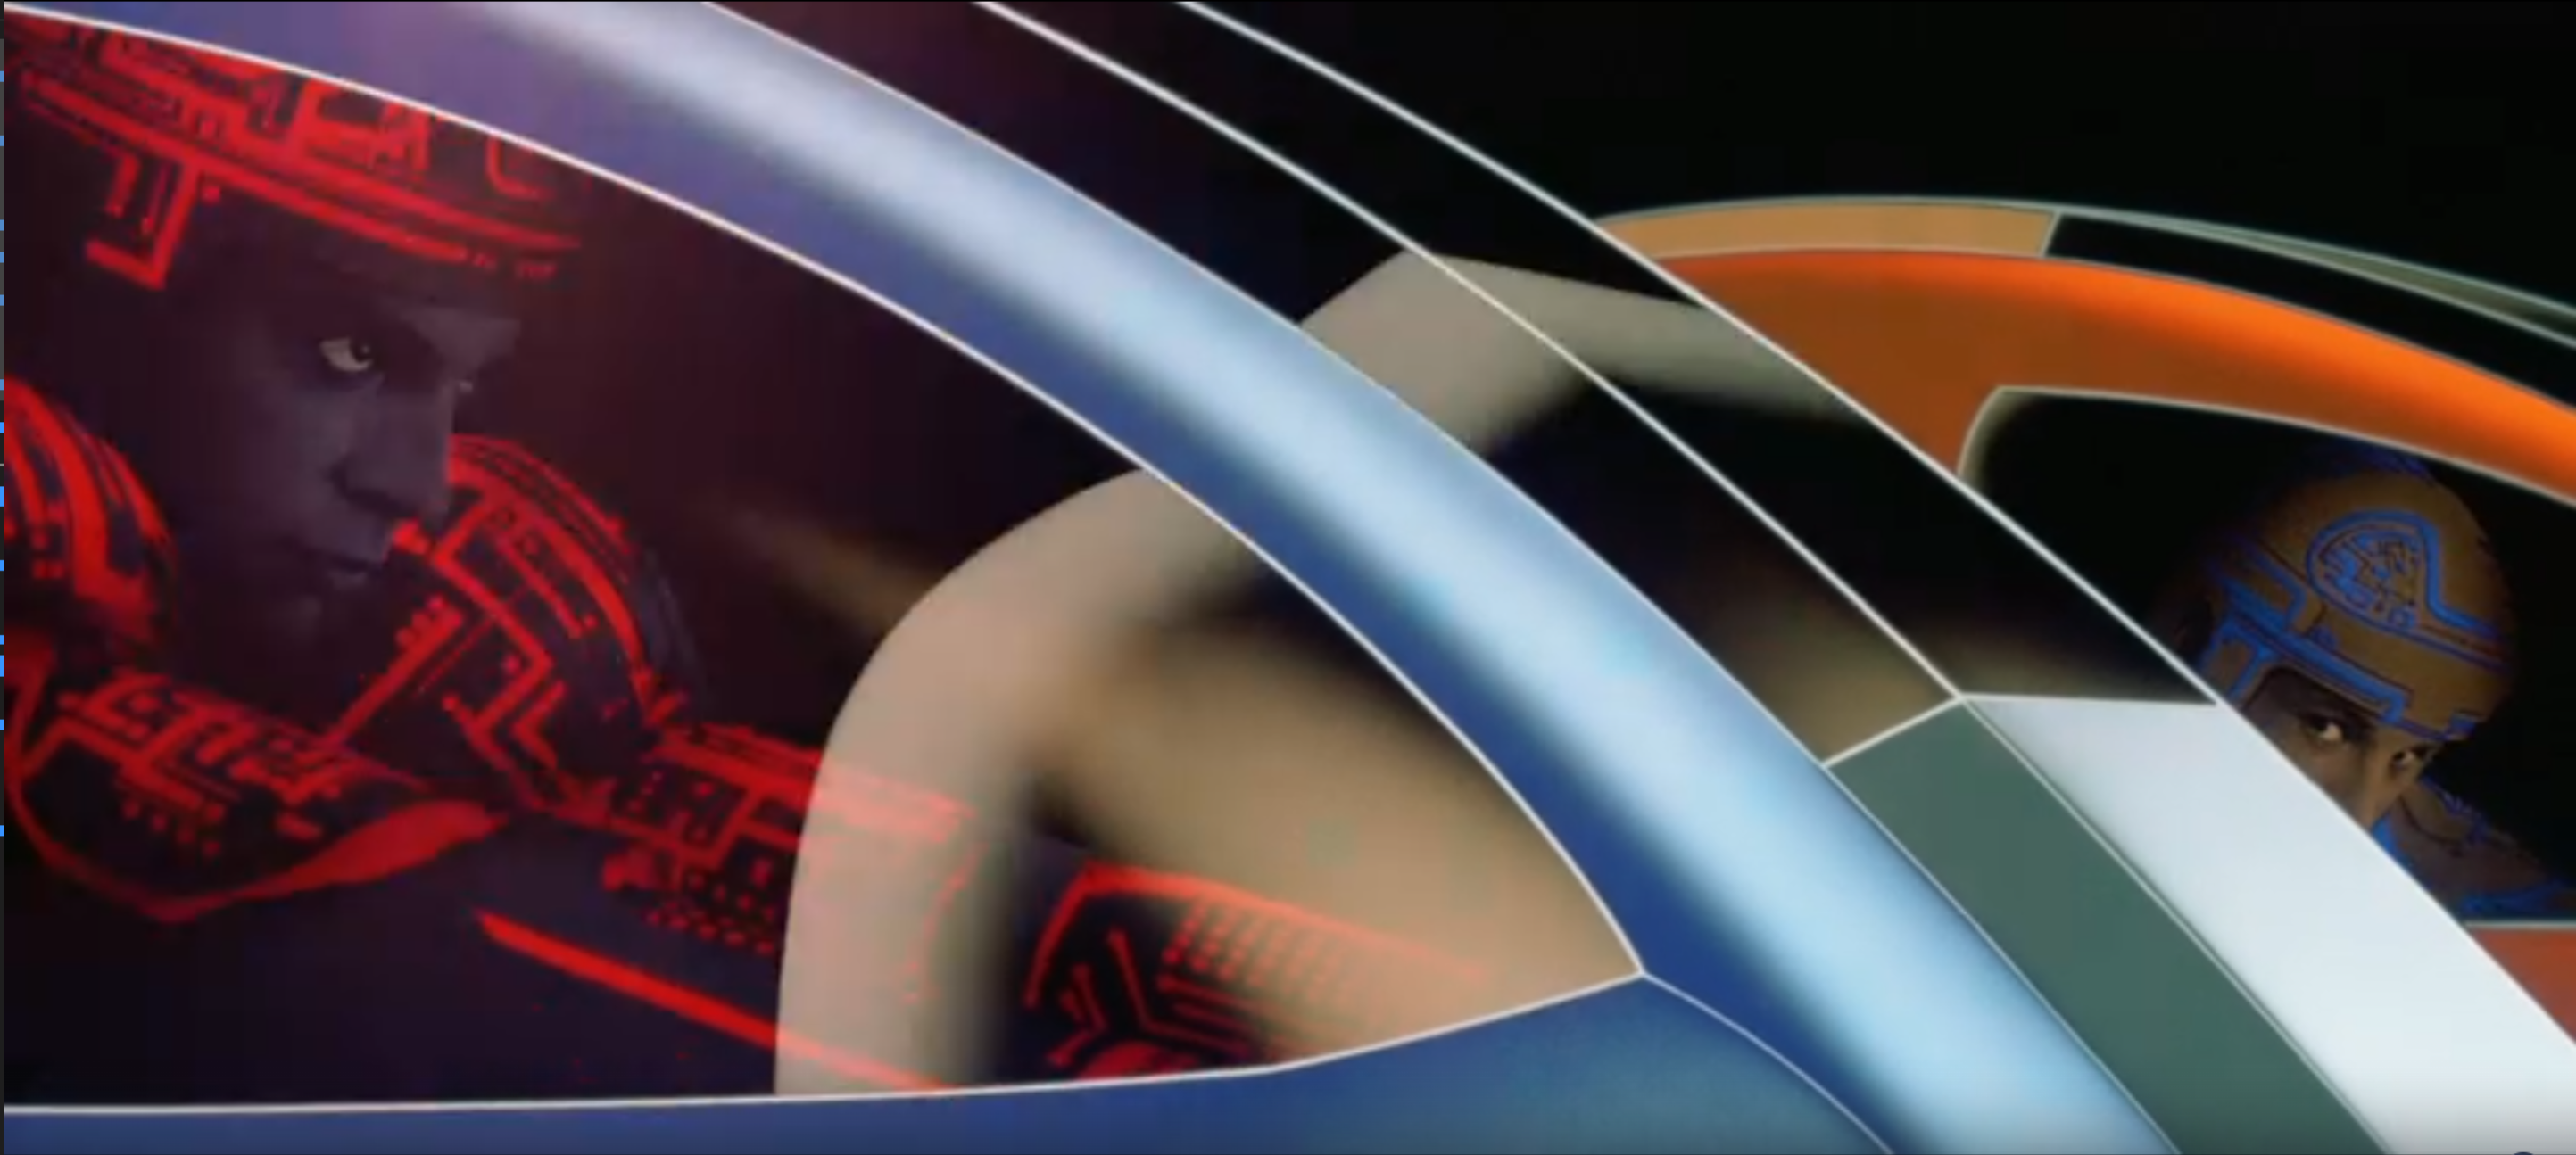
\includegraphics[width=\paperwidth, keepaspectratio]{static/img/tron.png}
    };

    \node[fill=black, opacity=1, minimum width=\paperwidth, text opacity=0.7,
          minimum height=2.5em, anchor=south, text=white, font=\large\bfseries] 
      at ([yshift=0em]current page.south) {Your data isn't just text anymore - it's vectors};
    
    \node[anchor=south east] at ([xshift=-0.5em, yshift=0em]current page.south east) {
      \includesvg[width=2em]{static/img/rabbit.svg}
    };

  \end{tikzpicture}
\end{frame}
    \section{Ряды}
      \subsection{введение}
        \begin{frame}
  \bfseries Опасности, которые нас подстерегают при хранении больших JSON в БД?
  \normalfont
  \vspace{1em}
  \begin{itemize}[leftmargin=1em,itemsep=0.7em, label=\RNDSmarker]
    \item рост объёма хранилища
    \item дорогие бэкапы и восстановление
    \item сложность анализа
    \item память и скорость в Rails
    \item редкое использование тяжёлых данных
  \end{itemize}
\end{frame}
      \subsection{о чем речь}
        \begin{frame}
  \bfseries Временной ряд определяется набором параметров:
  \normalfont
  \vspace{2em}
  \begin{itemize}[leftmargin=1em,itemsep=0.7em, label=\RNDSmarker]
    \item временная метка \textcolor{gray}{(01.01.2000, 946684800, 2000-01-01 00:00:00 UTC)}
    \item название статистики \textcolor{gray}{(загрузка CPU, количество заказов, количество кликов)}
    \item значение \textcolor{gray}{(67, 0.75, 156626)}
    \item набор признаков \textcolor{gray}{(host: 'home', region: 'Rostov-on-Don', browser: 'Chrome')}
  \end{itemize}
\end{frame}

      \subsection{tsdb}
        \begin{frame}
  \begin{columns} 
    \begin{column}{0.32\textwidth} 
      \begin{minipage}[\textheight]{\linewidth}
        \vspace{0.15\textheight} 
        \begin{tikzpicture} 
          \node[
            fill=RNDScardBody, 
            rounded corners=1em, 
            minimum width=\linewidth, minimum height=\linewidth, 
            align=center, 
            font=\ttfamily\color{RNDSorange}\LARGE\bfseries] (mainnode)
            {Victoria\\Metrics};
          \node[anchor=north east, xshift=3em, yshift=8] (icon) at (mainnode.north west) {
            \includesvg[width=3em]{static/img/victoriametrics.svg}
          }; 
        \end{tikzpicture} 
      \end{minipage} 
    \end{column} 
    \begin{column}{0.32\textwidth} 
      \begin{minipage}[\textheight]{\linewidth} 
        \vspace{0.15\textheight} 
        \begin{tikzpicture} 
          \node[
            fill=RNDScardBody, 
            rounded corners=1em, 
            minimum width=\linewidth, minimum height=\linewidth, 
            align=center, 
            font=\ttfamily\color{RNDSorange}\LARGE\bfseries] (mainnode)
            {InfluxDB};
          \node[anchor=north east, xshift=3em, yshift=8] (icon) at (mainnode.north west) {
            \includesvg[width=3em]{static/img/influxdb.svg}
          };
        \end{tikzpicture} 
      \end{minipage} 
    \end{column} 
    \begin{column}{0.32\textwidth} 
      \begin{minipage}[\textheight]{\linewidth} 
        \vspace{0.15\textheight} 
        \begin{tikzpicture} 
          \node[
            fill=RNDScardBody, 
            rounded corners=1em, 
            minimum width=\linewidth, minimum height=\linewidth, 
            align=center, 
            font=\ttfamily\color{RNDSorange}\LARGE\bfseries] (mainnode)
           {TimescaleDB};
           \node[
            star, star points=5, star point ratio=2.5, 
            fill=RNDSorange, minimum size=1em, scale=0.8, 
            anchor=north east, xshift=-1.5em, yshift=-1.5em
          ] at (mainnode.north east) {};
          \node[anchor=north east, xshift=3em, yshift=8] (icon) at (mainnode.north west) {
            \includesvg[width=3em]{static/img/timescale.svg}
          }; 
        \end{tikzpicture} 
      \end{minipage} 
    \end{column} 
  \end{columns} 
\end{frame}
      \subsection{timescaleDB}
        \begin{frame}
  \bfseries Что дает использование TimescaleDB
  \normalfont
  \vspace{1em}
  \begin{itemize}[leftmargin=1em,itemsep=0.7em, label=\RNDSmarker]
    \item быстрая вставка
    \item быстрая чтение
    \item retention policies
    \item сompression
    \item locf, interpolate, rate, delta, percentile\_agg, approx\_percentile
  \end{itemize}
\end{frame}


      \subsection{заключение}
        \begin{frame}[plain]
  \begin{tikzpicture}[remember picture, overlay]
    \node at (current page.center) {
      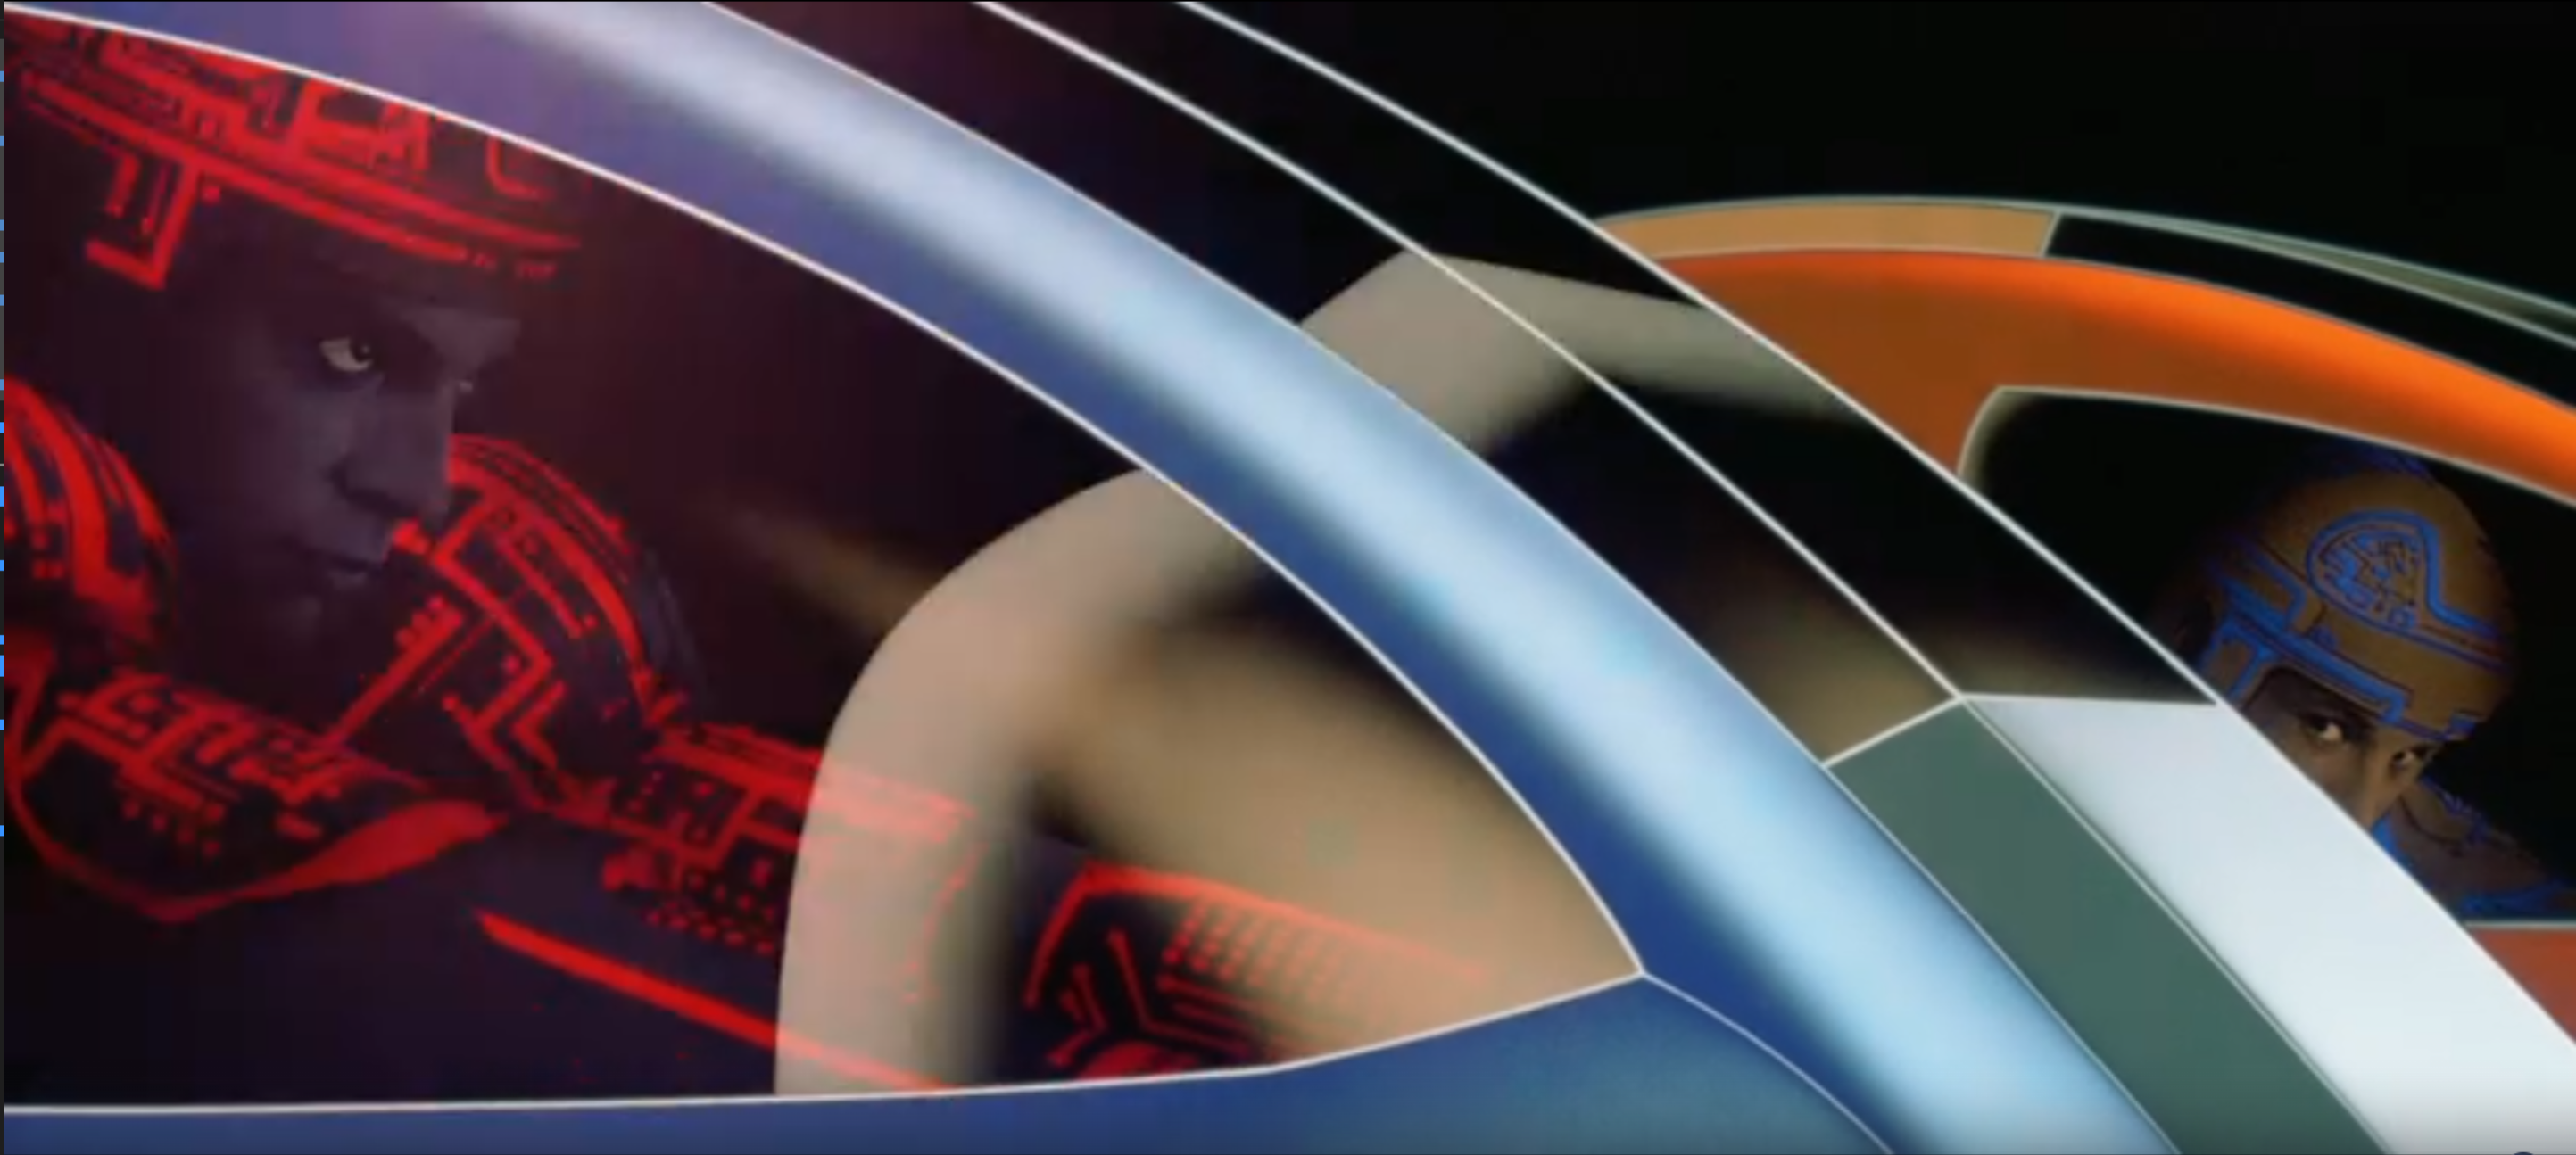
\includegraphics[width=\paperwidth, keepaspectratio]{static/img/tron.png}
    };

    \node[fill=black, opacity=1, minimum width=\paperwidth, text opacity=0.7,
          minimum height=2.5em, anchor=south, text=white, font=\large\bfseries] 
      at ([yshift=0em]current page.south) {Your data isn't just text anymore - it's vectors};
    
    \node[anchor=south east] at ([xshift=-0.5em, yshift=0em]current page.south east) {
      \includesvg[width=2em]{static/img/rabbit.svg}
    };

  \end{tikzpicture}
\end{frame}
    \section{ExternalHash}
      \subsection{введение}
        \begin{frame}
  \bfseries Опасности, которые нас подстерегают при хранении больших JSON в БД?
  \normalfont
  \vspace{1em}
  \begin{itemize}[leftmargin=1em,itemsep=0.7em, label=\RNDSmarker]
    \item рост объёма хранилища
    \item дорогие бэкапы и восстановление
    \item сложность анализа
    \item память и скорость в Rails
    \item редкое использование тяжёлых данных
  \end{itemize}
\end{frame}
      \subsection{о чем речь}
        \begin{frame}
  \bfseries Чего хотелось бы
  \normalfont
  \vspace{1em}
  \begin{itemize}[leftmargin=1em,itemsep=0.7em, label=\RNDSmarker]
    \item чтобы JSON не занимали место в БД
    \item не ломать существующий интерфейс
    \item чтобы, при необходимости, данные могли храниться в БД
  \end{itemize}
\end{frame}
      \subsection{реализация}
        \begin{frame}[fragile, t]
  \begin{onlyenv}<1>
    \vspace{2em}
    \scalebox{0.7}{
      % \fontsize{7}{9}\selectfont % Компактный шрифт
      \begin{sequencediagram}
        \tikzset{
          inststyle/.append style={
            drop shadow={opacity=1.0,fill=RNDSorange}
          }
        }
        \newinst {app}{AbstractClient}
        \newinst [1]{model}{ActiveRecord}
        \newinst [3]{db}{PostgreSQL}
        \newinst [1]{s3}{S3 storrage}
        \begin{sdblock}{alt}{JSON in PostgreSQL}
          \begin{call}{model}{SELECT id, data FROM record}{db}{42, \{"name": "Иван"\}}
          \end{call}
          \begin{call}{app}{model.datap['name']}{model}{"Иван"}
            \begin{call}{model}{external?}{model}{false}
            \end{call}
          \end{call}
        \end{sdblock}
      \end{sequencediagram}   
    }
  \end{onlyenv}
  \begin{onlyenv}<2>
    \vspace{2em}
    \scalebox{0.7}{
      % \fontsize{7}{9}\selectfont % Компактный шрифт
      \begin{sequencediagram}
        \tikzset{
          inststyle/.append style={
            drop shadow={opacity=1.0,fill=RNDSorange}
          },
        }
        \newinst {app}{AbstractClient}
        \newinst [1]{model}{ActiveRecord}
        \newinst [3]{db}{PostgreSQL}
        \newinst [1]{s3}{S3 storrage}
        \begin{sdblock}{alt}{JSON in S3 storrage}
          \begin{call}{model}{SELECT id, data FROM record}{db}{\{"external": true, "uuid": "111"\}}
          \end{call}
          \begin{call}{app}{model.datap['name']}{model}{"Иван"}
            \begin{call}{model}{external?}{model}{true}
            \end{call}
            \begin{call}{model}{GET /bucket/path/111.json}{s3}{\{"name": "Иван"\}}
            \end{call}
            \begin{call}{model}{Парсинг JSON в Hash}{model}{}
            \end{call}
          \end{call}
        \end{sdblock}
      \end{sequencediagram}   
    }
  \end{onlyenv}
  \begin{onlyenv}<3>
    \begin{tcblisting}{
      listing engine=minted,
      minted language=ruby,
      minted options={fontsize=\footnotesize, linenos=true, numbersep=5pt},
      colback=RNDScardBody,
      colframe=RNDSorange,
      listing only,
      title=MaybeExternalHash,
      fonttitle=\normalsize,
    }
class MaybeExternalHash < ActiveSupport::Hash
  class ExternalHash
    
    def initialize(file)
      @file = file
    end
    
    def to_hash
      @hash ||= JSON.load(@file)
    end
    
    def query(path, &)
      Parser.parse(@file, path)
    end
  end
  \end{tcblisting}

  \end{onlyenv}
  \begin{onlyenv}<4>
    \begin{tcblisting}{
      listing engine=minted,
      minted language=ruby,
      minted options={fontsize=\footnotesize, linenos=true, numbersep=5pt},
      colback=RNDScardBody,
      colframe=RNDSorange,
      listing only,
      title=MaybeExternalHash,
      fonttitle=\normalsize,
    }
class MaybeExternalHash < ActiveSupport::Hash

  def download
    return unless external?
    file = Loader.get(external_uuid)
    ExternalHash.new(file[:file])
  end

  def [](key)
    if external?
      get_data_from_external(key.to_s)
    else
      super
    end
  end
  \end{tcblisting}

  \end{onlyenv}
  \begin{onlyenv}<5>
    \begin{tcblisting}{
      listing engine=minted,
      minted language=ruby,
      minted options={fontsize=\footnotesize, linenos=true, numbersep=5pt},
      colback=RNDScardBody,
      colframe=RNDSorange,
      listing only,
      title=MaybeExternalHash,
      fonttitle=\normalsize,
    }
class MaybeExternalHash < ActiveSupport::Hash

  def get_data_from_external(path)
    return nil unless external?
    @hash ||= self.download
    value = @hash.query(path)
  end

  def external?
    self.class.superclass.instance_method(:[]).bind(self).call(:external)
  end

  def external_uuid
  end
  \end{tcblisting}

  \end{onlyenv}
\end{frame}
      \subsection{+/-}
        \begin{frame}
  \bfseries Плюсы
  \normalfont
  \vspace{1em}
  \begin{itemize}[leftmargin=1em,itemsep=0.7em, label=\RNDSmarker]
    \item существенное сокращение размера БД
    \item скорость выборок из БД
  \end{itemize}
  \vspace{2em}
  \bfseries Минусы
  \normalfont
  \vspace{1em}
  \begin{itemize}[leftmargin=1em,itemsep=0.7em, label=\RNDSmarkerGray]
    \item лишние сетевые запросы
    \item медленный доступ к данным
  \end{itemize}
\end{frame}
      \subsection{заключение}
        \begin{frame}[plain]
  \begin{tikzpicture}[remember picture, overlay]
    \node at (current page.center) {
      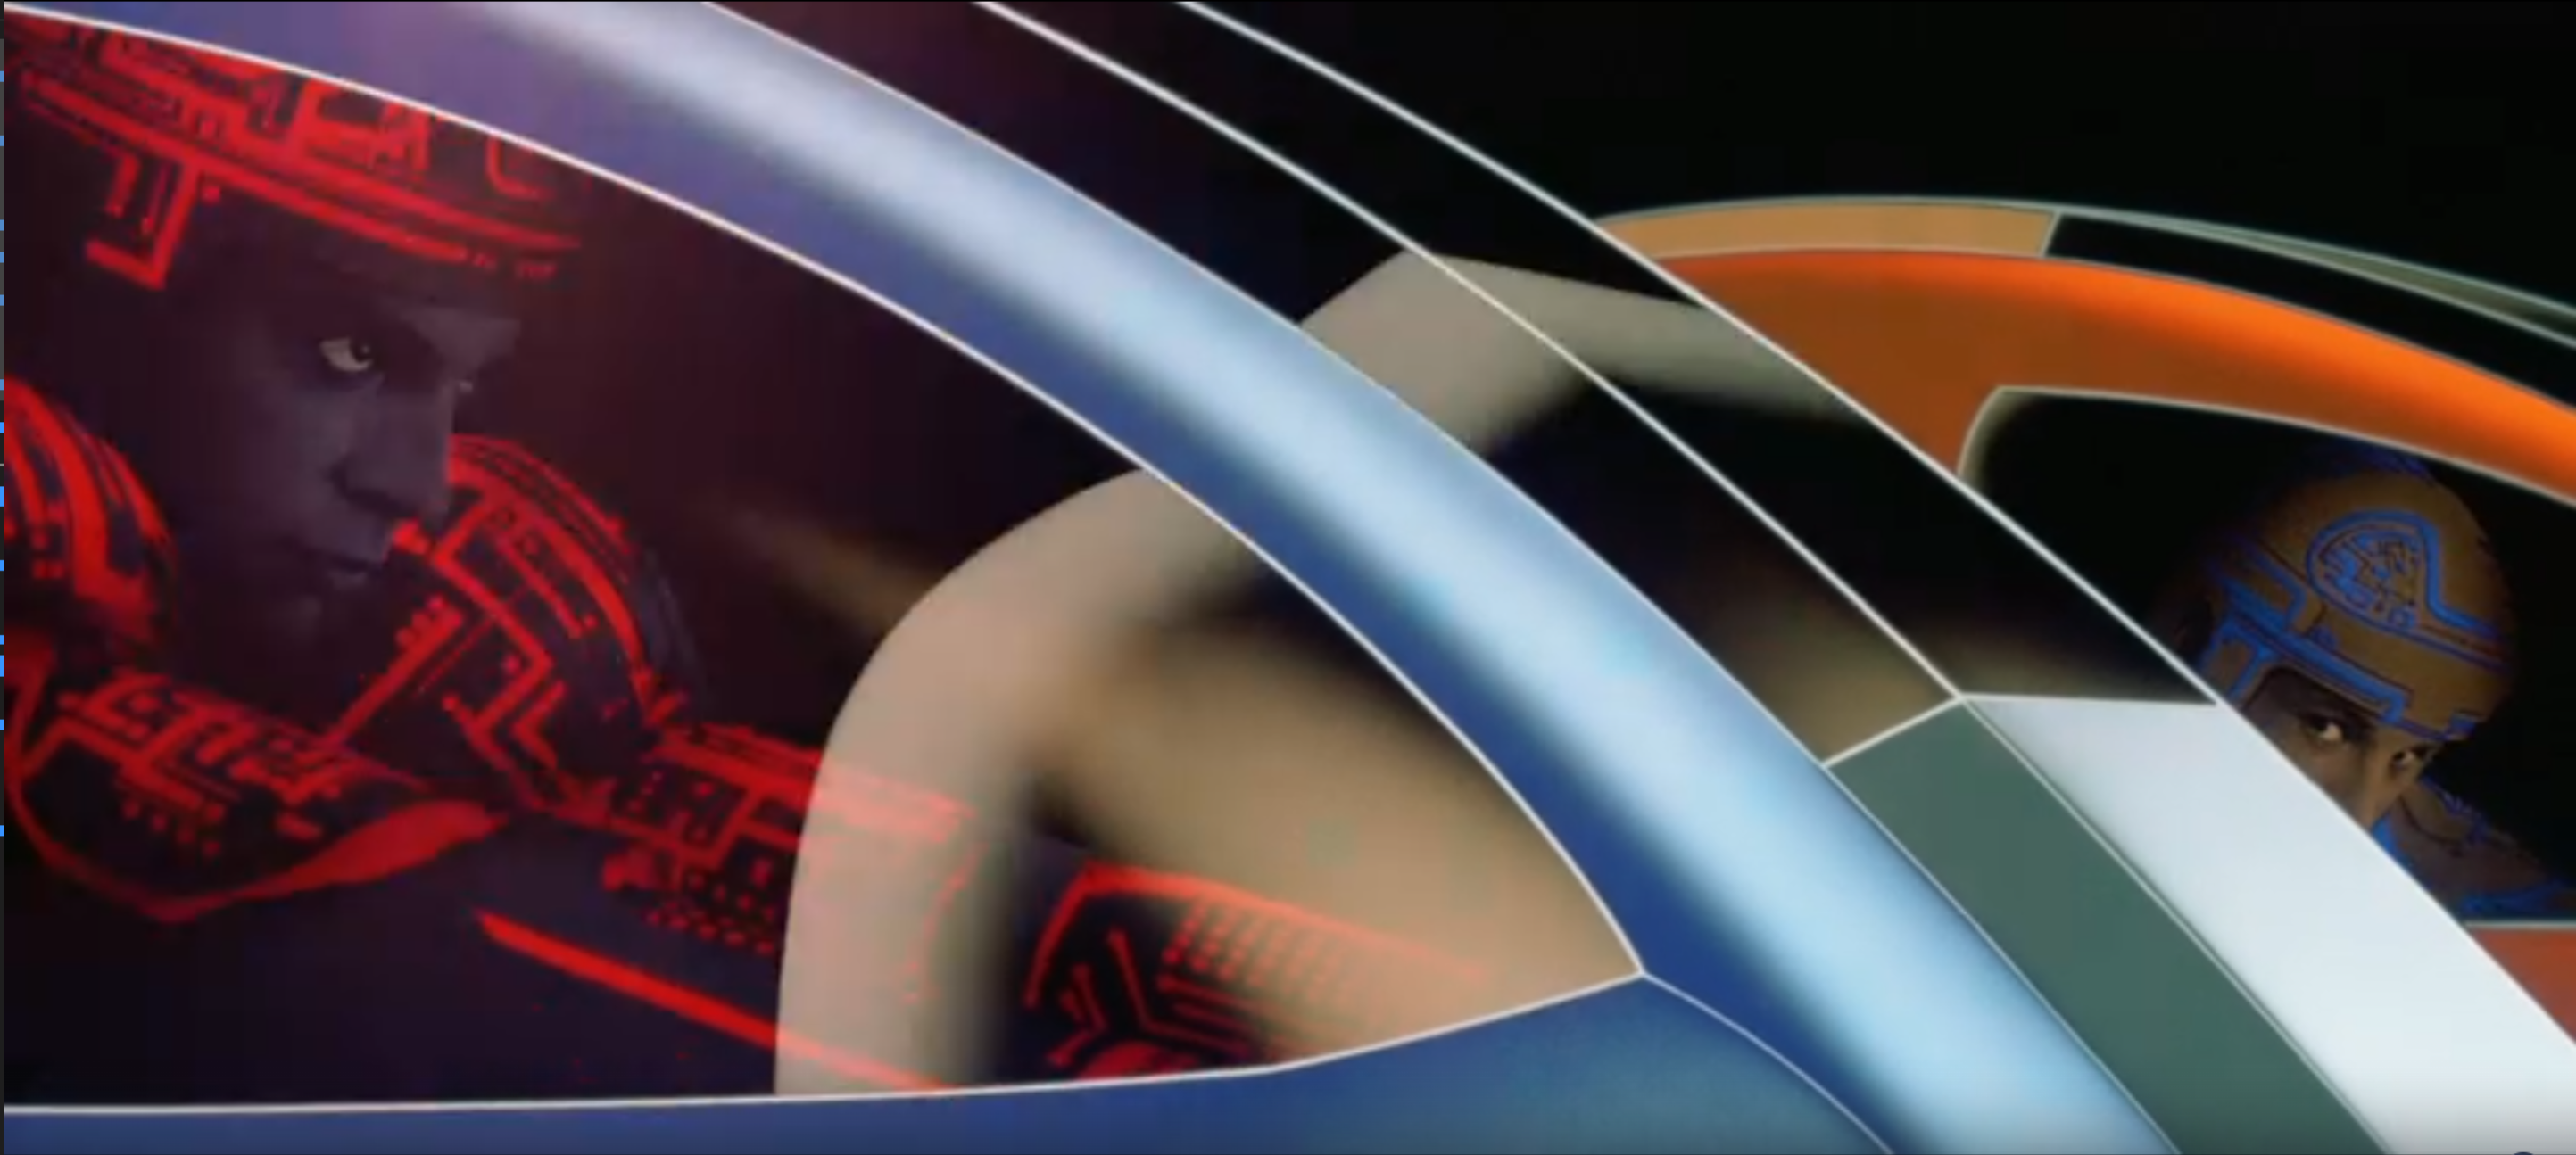
\includegraphics[width=\paperwidth, keepaspectratio]{static/img/tron.png}
    };

    \node[fill=black, opacity=1, minimum width=\paperwidth, text opacity=0.7,
          minimum height=2.5em, anchor=south, text=white, font=\large\bfseries] 
      at ([yshift=0em]current page.south) {Your data isn't just text anymore - it's vectors};
    
    \node[anchor=south east] at ([xshift=-0.5em, yshift=0em]current page.south east) {
      \includesvg[width=2em]{static/img/rabbit.svg}
    };

  \end{tikzpicture}
\end{frame}
  \part{Заключение}
    \section{Заключение}
      \begin{frame}
  \centering
  \bfseries\LARGE ВОПРОСЫ
\end{frame}

\end{document}